\documentclass[1p]{elsarticle_modified}
%\bibliographystyle{elsarticle-num}

%\usepackage[colorlinks]{hyperref}
%\usepackage{abbrmath_seonhwa} %\Abb, \Ascr, \Acal ,\Abf, \Afrak
\usepackage{amsfonts}
\usepackage{amssymb}
\usepackage{amsmath}
\usepackage{amsthm}
\usepackage{scalefnt}
\usepackage{amsbsy}
\usepackage{kotex}
\usepackage{caption}
\usepackage{subfig}
\usepackage{color}
\usepackage{graphicx}
\usepackage{xcolor} %% white, black, red, green, blue, cyan, magenta, yellow
\usepackage{float}
\usepackage{setspace}
\usepackage{hyperref}

\usepackage{tikz}
\usetikzlibrary{arrows}

\usepackage{multirow}
\usepackage{array} % fixed length table
\usepackage{hhline}

%%%%%%%%%%%%%%%%%%%%%
\makeatletter
\renewcommand*\env@matrix[1][\arraystretch]{%
	\edef\arraystretch{#1}%
	\hskip -\arraycolsep
	\let\@ifnextchar\new@ifnextchar
	\array{*\c@MaxMatrixCols c}}
\makeatother %https://tex.stackexchange.com/questions/14071/how-can-i-increase-the-line-spacing-in-a-matrix
%%%%%%%%%%%%%%%

\usepackage[normalem]{ulem}

\newcommand{\msout}[1]{\ifmmode\text{\sout{\ensuremath{#1}}}\else\sout{#1}\fi}
%SOURCE: \msout is \stkout macro in https://tex.stackexchange.com/questions/20609/strikeout-in-math-mode

\newcommand{\cancel}[1]{
	\ifmmode
	{\color{red}\msout{#1}}
	\else
	{\color{red}\sout{#1}}
	\fi
}

\newcommand{\add}[1]{
	{\color{blue}\uwave{#1}}
}

\newcommand{\replace}[2]{
	\ifmmode
	{\color{red}\msout{#1}}{\color{blue}\uwave{#2}}
	\else
	{\color{red}\sout{#1}}{\color{blue}\uwave{#2}}
	\fi
}

\newcommand{\Sol}{\mathcal{S}} %segment
\newcommand{\D}{D} %diagram
\newcommand{\A}{\mathcal{A}} %arc


%%%%%%%%%%%%%%%%%%%%%%%%%%%%%5 test

\def\sl{\operatorname{\textup{SL}}(2,\Cbb)}
\def\psl{\operatorname{\textup{PSL}}(2,\Cbb)}
\def\quan{\mkern 1mu \triangleright \mkern 1mu}

\theoremstyle{definition}
\newtheorem{thm}{Theorem}[section]
\newtheorem{prop}[thm]{Proposition}
\newtheorem{lem}[thm]{Lemma}
\newtheorem{ques}[thm]{Question}
\newtheorem{cor}[thm]{Corollary}
\newtheorem{defn}[thm]{Definition}
\newtheorem{exam}[thm]{Example}
\newtheorem{rmk}[thm]{Remark}
\newtheorem{alg}[thm]{Algorithm}

\newcommand{\I}{\sqrt{-1}}
\begin{document}

%\begin{frontmatter}
%
%\title{Boundary parabolic representations of knots up to 8 crossings}
%
%%% Group authors per affiliation:
%\author{Yunhi Cho} 
%\address{Department of Mathematics, University of Seoul, Seoul, Korea}
%\ead{yhcho@uos.ac.kr}
%
%
%\author{Seonhwa Kim} %\fnref{s_kim}}
%\address{Center for Geometry and Physics, Institute for Basic Science, Pohang, 37673, Korea}
%\ead{ryeona17@ibs.re.kr}
%
%\author{Hyuk Kim}
%\address{Department of Mathematical Sciences, Seoul National University, Seoul 08826, Korea}
%\ead{hyukkim@snu.ac.kr}
%
%\author{Seokbeom Yoon}
%\address{Department of Mathematical Sciences, Seoul National University, Seoul, 08826,  Korea}
%\ead{sbyoon15@snu.ac.kr}
%
%\begin{abstract}
%We find all boundary parabolic representation of knots up to 8 crossings.
%
%\end{abstract}
%\begin{keyword}
%    \MSC[2010] 57M25 
%\end{keyword}
%
%\end{frontmatter}

%\linenumbers
%\tableofcontents
%
\newcommand\colored[1]{\textcolor{white}{\rule[-0.35ex]{0.8em}{1.4ex}}\kern-0.8em\color{red} #1}%
%\newcommand\colored[1]{\textcolor{white}{ #1}\kern-2.17ex	\textcolor{white}{ #1}\kern-1.81ex	\textcolor{white}{ #1}\kern-2.15ex\color{red}#1	}

{\Large $\underline{11a_{117}~(K11a_{117})}$}

\setlength{\tabcolsep}{10pt}
\renewcommand{\arraystretch}{1.6}
\vspace{1cm}\begin{tabular}{m{100pt}>{\centering\arraybackslash}m{274pt}}
\multirow{5}{120pt}{
	\centering
	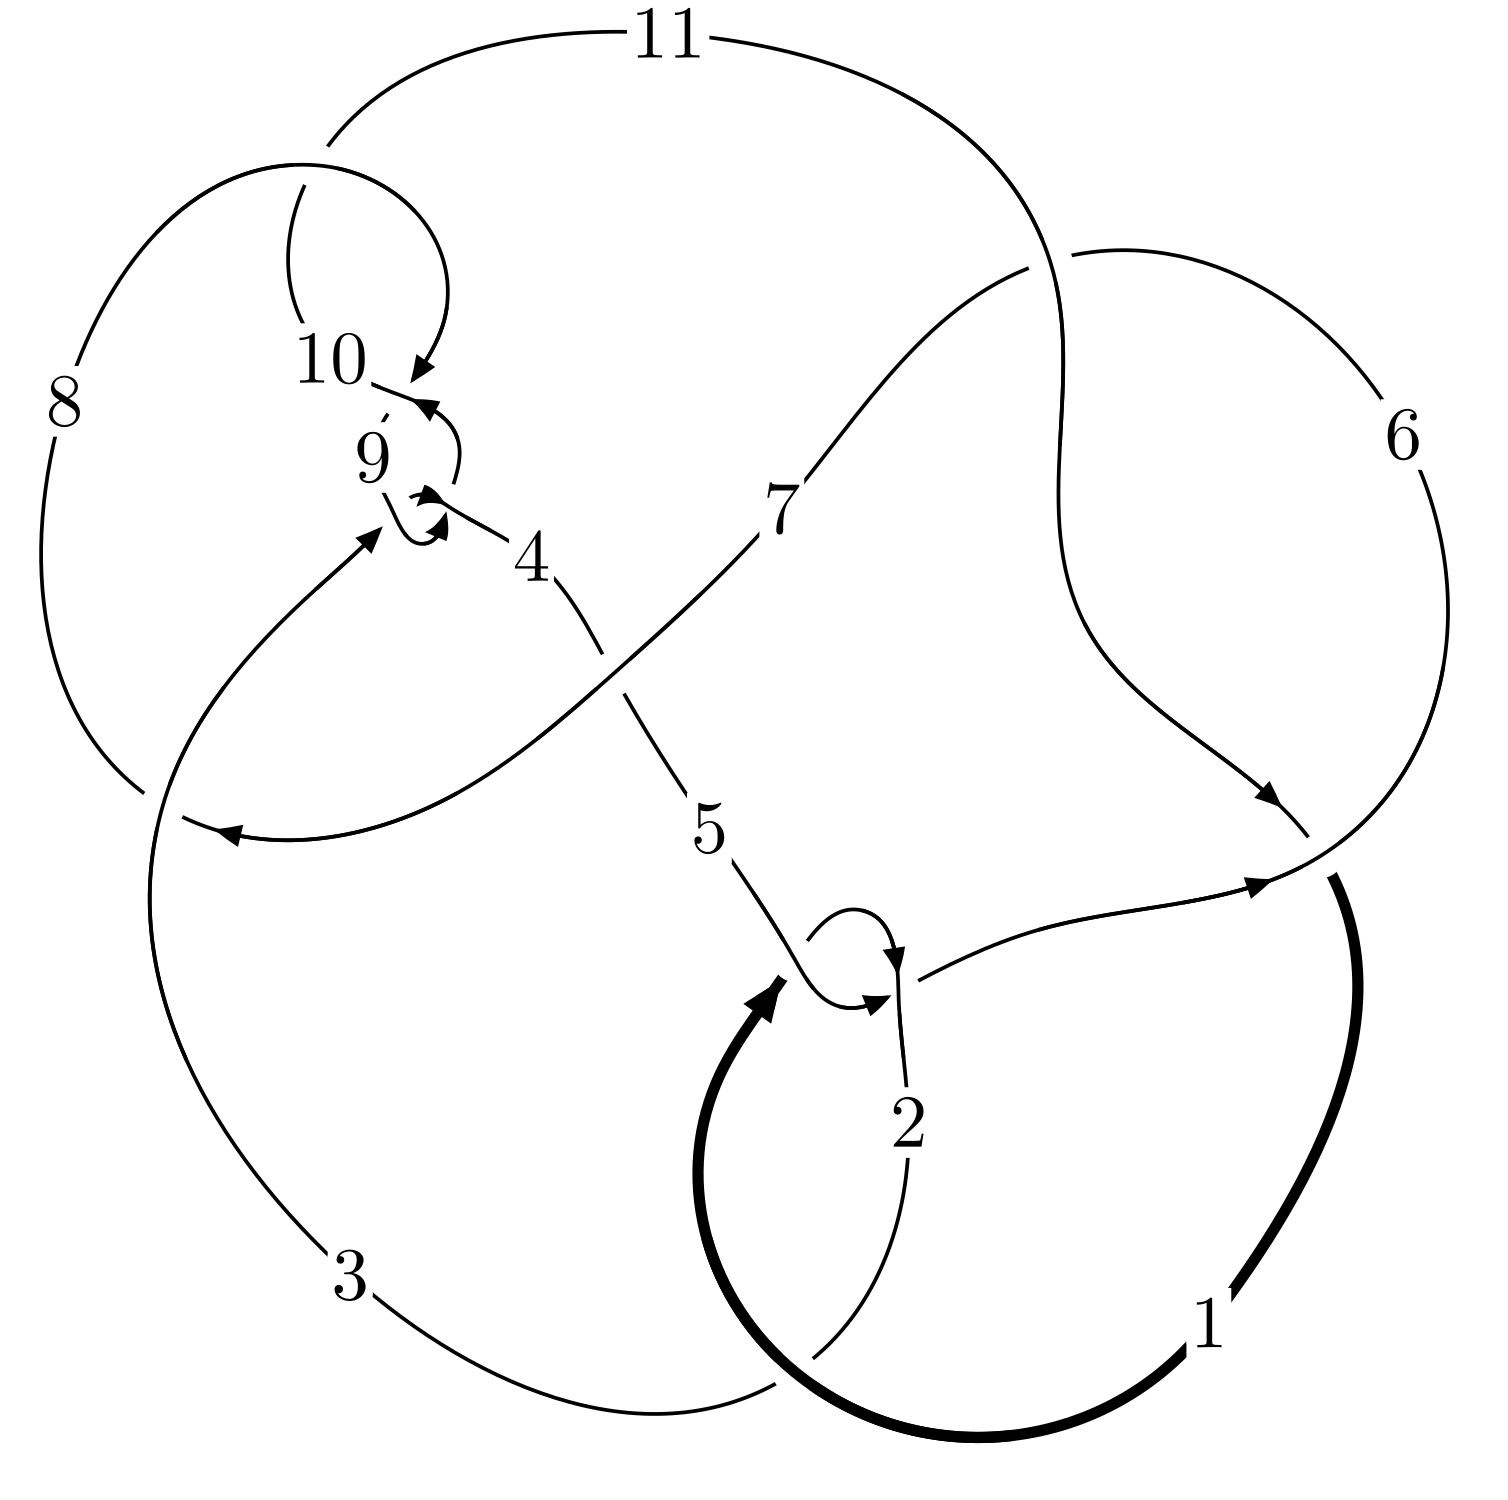
\includegraphics[width=112pt]{../../../GIT/diagram.site/Diagrams/png/366_11a_117.png}\\
\ \ \ A knot diagram\footnotemark}&
\allowdisplaybreaks
\textbf{Linearized knot diagam} \\
\cline{2-2}
 &
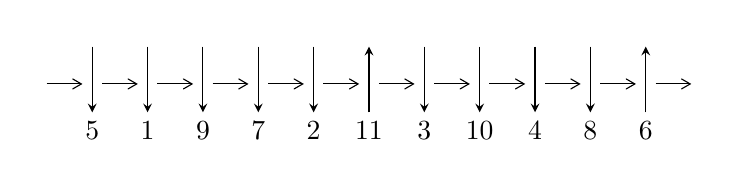
\begin{tikzpicture}[x=20pt, y=17pt]
	% nodes
	\node (C0) at (0, 0) {};
	\node (C1) at (1, 0) {};
	\node (C1U) at (1, +1) {};
	\node (C1D) at (1, -1) {5};

	\node (C2) at (2, 0) {};
	\node (C2U) at (2, +1) {};
	\node (C2D) at (2, -1) {1};

	\node (C3) at (3, 0) {};
	\node (C3U) at (3, +1) {};
	\node (C3D) at (3, -1) {9};

	\node (C4) at (4, 0) {};
	\node (C4U) at (4, +1) {};
	\node (C4D) at (4, -1) {7};

	\node (C5) at (5, 0) {};
	\node (C5U) at (5, +1) {};
	\node (C5D) at (5, -1) {2};

	\node (C6) at (6, 0) {};
	\node (C6U) at (6, +1) {};
	\node (C6D) at (6, -1) {11};

	\node (C7) at (7, 0) {};
	\node (C7U) at (7, +1) {};
	\node (C7D) at (7, -1) {3};

	\node (C8) at (8, 0) {};
	\node (C8U) at (8, +1) {};
	\node (C8D) at (8, -1) {10};

	\node (C9) at (9, 0) {};
	\node (C9U) at (9, +1) {};
	\node (C9D) at (9, -1) {4};

	\node (C10) at (10, 0) {};
	\node (C10U) at (10, +1) {};
	\node (C10D) at (10, -1) {8};

	\node (C11) at (11, 0) {};
	\node (C11U) at (11, +1) {};
	\node (C11D) at (11, -1) {6};
	\node (C12) at (12, 0) {};

	% arrows
	\draw[->,>={angle 60}]
	(C0) edge (C1) (C1) edge (C2) (C2) edge (C3) (C3) edge (C4) (C4) edge (C5) (C5) edge (C6) (C6) edge (C7) (C7) edge (C8) (C8) edge (C9) (C9) edge (C10) (C10) edge (C11) (C11) edge (C12) ;	\draw[->,>=stealth]
	(C1U) edge (C1D) (C2U) edge (C2D) (C3U) edge (C3D) (C4U) edge (C4D) (C5U) edge (C5D) (C6D) edge (C6U) (C7U) edge (C7D) (C8U) edge (C8D) (C9U) edge (C9D) (C10U) edge (C10D) (C11D) edge (C11U) ;
	\end{tikzpicture} \\
\hhline{~~} \\& 
\textbf{Solving Sequence} \\ \cline{2-2} 
 &
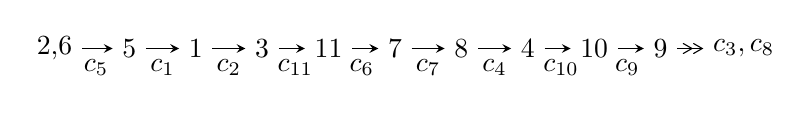
\begin{tikzpicture}[x=24pt, y=7pt]
	% node
	\node (A0) at (-1/8, 0) {2,6};
	\node (A1) at (1, 0) {5};
	\node (A2) at (2, 0) {1};
	\node (A3) at (3, 0) {3};
	\node (A4) at (4, 0) {11};
	\node (A5) at (5, 0) {7};
	\node (A6) at (6, 0) {8};
	\node (A7) at (7, 0) {4};
	\node (A8) at (8, 0) {10};
	\node (A9) at (9, 0) {9};
	\node (C1) at (1/2, -1) {$c_{5}$};
	\node (C2) at (3/2, -1) {$c_{1}$};
	\node (C3) at (5/2, -1) {$c_{2}$};
	\node (C4) at (7/2, -1) {$c_{11}$};
	\node (C5) at (9/2, -1) {$c_{6}$};
	\node (C6) at (11/2, -1) {$c_{7}$};
	\node (C7) at (13/2, -1) {$c_{4}$};
	\node (C8) at (15/2, -1) {$c_{10}$};
	\node (C9) at (17/2, -1) {$c_{9}$};
	\node (A10) at (41/4, 0) {$c_{3},c_{8}$};

	% edge
	\draw[->,>=stealth]	
	(A0) edge (A1) (A1) edge (A2) (A2) edge (A3) (A3) edge (A4) (A4) edge (A5) (A5) edge (A6) (A6) edge (A7) (A7) edge (A8) (A8) edge (A9) ;
	\draw[->>,>={angle 60}]	
	(A9) edge (A10);
\end{tikzpicture} \\ 

\end{tabular} \\

\footnotetext{
The image of knot diagram is generated by the software ``\textbf{Draw programme}" developed by Andrew Bartholomew(\url{http://www.layer8.co.uk/maths/draw/index.htm\#Running-draw}), where we modified some parts for our purpose(\url{https://github.com/CATsTAILs/LinksPainter}).
}\phantom \\ \newline 
\centering \textbf{Ideals for irreducible components\footnotemark of $X_{\text{par}}$} 
 
\begin{align*}
I^u_{1}&=\langle 
u^{57}-2 u^{56}+\cdots+4 u-1\rangle \\
I^u_{2}&=\langle 
u+1\rangle \\
\\
\end{align*}
\raggedright * 2 irreducible components of $\dim_{\mathbb{C}}=0$, with total 58 representations.\\
\footnotetext{All coefficients of polynomials are rational numbers. But the coefficients are sometimes approximated in decimal forms when there is not enough margin.}
\newpage
\renewcommand{\arraystretch}{1}
\centering \section*{I. $I^u_{1}= \langle u^{57}-2 u^{56}+\cdots+4 u-1 \rangle$}
\flushleft \textbf{(i) Arc colorings}\\
\begin{tabular}{m{7pt} m{180pt} m{7pt} m{180pt} }
\flushright $a_{2}=$&$\begin{pmatrix}0\\u\end{pmatrix}$ \\
\flushright $a_{6}=$&$\begin{pmatrix}1\\0\end{pmatrix}$ \\
\flushright $a_{5}=$&$\begin{pmatrix}1\\- u^2\end{pmatrix}$ \\
\flushright $a_{1}=$&$\begin{pmatrix}u\\- u^3+u\end{pmatrix}$ \\
\flushright $a_{3}=$&$\begin{pmatrix}- u^3\\u^5- u^3+u\end{pmatrix}$ \\
\flushright $a_{11}=$&$\begin{pmatrix}u^3\\- u^3+u\end{pmatrix}$ \\
\flushright $a_{7}=$&$\begin{pmatrix}u^6- u^4+1\\- u^6+2 u^4- u^2\end{pmatrix}$ \\
\flushright $a_{8}=$&$\begin{pmatrix}- u^{14}+3 u^{12}-4 u^{10}+u^8+2 u^6-2 u^4+1\\u^{16}-4 u^{14}+8 u^{12}-8 u^{10}+4 u^8\end{pmatrix}$ \\
\flushright $a_{4}=$&$\begin{pmatrix}- u^{14}+3 u^{12}-4 u^{10}+u^8+2 u^6-2 u^4+1\\u^{14}-4 u^{12}+7 u^{10}-6 u^8+2 u^6- u^2\end{pmatrix}$ \\
\flushright $a_{10}=$&$\begin{pmatrix}u^{33}-8 u^{31}+\cdots-4 u^5+u\\- u^{35}+9 u^{33}+\cdots- u^3+u\end{pmatrix}$ \\
\flushright $a_{9}=$&$\begin{pmatrix}- u^{52}+13 u^{50}+\cdots+u^2+1\\u^{54}-14 u^{52}+\cdots-2 u^4+u^2\end{pmatrix}$\\ \flushright $a_{9}=$&$\begin{pmatrix}- u^{52}+13 u^{50}+\cdots+u^2+1\\u^{54}-14 u^{52}+\cdots-2 u^4+u^2\end{pmatrix}$\\&\end{tabular}
\flushleft \textbf{(ii) Obstruction class $= -1$}\\~\\
\flushleft \textbf{(iii) Cusp Shapes $= -8 u^{56}+12 u^{55}+\cdots+36 u-22$}\\~\\
\newpage\renewcommand{\arraystretch}{1}
\flushleft \textbf{(iv) u-Polynomials at the component}\newline \\
\begin{tabular}{m{50pt}|m{274pt}}
Crossings & \hspace{64pt}u-Polynomials at each crossing \\
\hline $$\begin{aligned}c_{1},c_{5}\end{aligned}$$&$\begin{aligned}
&u^{57}+2 u^{56}+\cdots+4 u+1
\end{aligned}$\\
\hline $$\begin{aligned}c_{2}\end{aligned}$$&$\begin{aligned}
&u^{57}+30 u^{56}+\cdots+2 u+1
\end{aligned}$\\
\hline $$\begin{aligned}c_{3},c_{9}\end{aligned}$$&$\begin{aligned}
&u^{57}-9 u^{55}+\cdots+2 u+1
\end{aligned}$\\
\hline $$\begin{aligned}c_{4}\end{aligned}$$&$\begin{aligned}
&u^{57}-8 u^{56}+\cdots+4 u+5
\end{aligned}$\\
\hline $$\begin{aligned}c_{6},c_{11}\end{aligned}$$&$\begin{aligned}
&u^{57}+3 u^{56}+\cdots+192 u+23
\end{aligned}$\\
\hline $$\begin{aligned}c_{7}\end{aligned}$$&$\begin{aligned}
&u^{57}+2 u^{56}+\cdots+170 u+25
\end{aligned}$\\
\hline $$\begin{aligned}c_{8},c_{10}\end{aligned}$$&$\begin{aligned}
&u^{57}+18 u^{56}+\cdots+2 u+1
\end{aligned}$\\
\hline
\end{tabular}\\~\\
\newpage\renewcommand{\arraystretch}{1}
\flushleft \textbf{(v) Riley Polynomials at the component}\newline \\
\begin{tabular}{m{50pt}|m{274pt}}
Crossings & \hspace{64pt}Riley Polynomials at each crossing \\
\hline $$\begin{aligned}c_{1},c_{5}\end{aligned}$$&$\begin{aligned}
&y^{57}-30 y^{56}+\cdots+2 y-1
\end{aligned}$\\
\hline $$\begin{aligned}c_{2}\end{aligned}$$&$\begin{aligned}
&y^{57}-6 y^{56}+\cdots+10 y-1
\end{aligned}$\\
\hline $$\begin{aligned}c_{3},c_{9}\end{aligned}$$&$\begin{aligned}
&y^{57}-18 y^{56}+\cdots+2 y-1
\end{aligned}$\\
\hline $$\begin{aligned}c_{4}\end{aligned}$$&$\begin{aligned}
&y^{57}+6 y^{56}+\cdots-1114 y-25
\end{aligned}$\\
\hline $$\begin{aligned}c_{6},c_{11}\end{aligned}$$&$\begin{aligned}
&y^{57}+45 y^{56}+\cdots-20314 y-529
\end{aligned}$\\
\hline $$\begin{aligned}c_{7}\end{aligned}$$&$\begin{aligned}
&y^{57}-6 y^{56}+\cdots+20350 y-625
\end{aligned}$\\
\hline $$\begin{aligned}c_{8},c_{10}\end{aligned}$$&$\begin{aligned}
&y^{57}+42 y^{56}+\cdots+26 y-1
\end{aligned}$\\
\hline
\end{tabular}\\~\\
\newpage\flushleft \textbf{(vi) Complex Volumes and Cusp Shapes}
$$\begin{array}{c|c|c}  
\text{Solutions to }I^u_{1}& \I (\text{vol} + \sqrt{-1}CS) & \text{Cusp shape}\\
 \hline 
\begin{aligned}
u &= -0.836048 + 0.550317 I\end{aligned}
 & \phantom{-}4.33306 + 3.41463 I & -2.47924 - 4.18588 I \\ \hline\begin{aligned}
u &= -0.836048 - 0.550317 I\end{aligned}
 & \phantom{-}4.33306 - 3.41463 I & -2.47924 + 4.18588 I \\ \hline\begin{aligned}
u &= \phantom{-}0.871162 + 0.481731 I\end{aligned}
 & -1.78928 - 4.12553 I & -10.51550 + 7.67121 I \\ \hline\begin{aligned}
u &= \phantom{-}0.871162 - 0.481731 I\end{aligned}
 & -1.78928 + 4.12553 I & -10.51550 - 7.67121 I \\ \hline\begin{aligned}
u &= \phantom{-}0.976200 + 0.175447 I\end{aligned}
 & -0.260427 - 0.093386 I & -10.10428 + 0.75716 I \\ \hline\begin{aligned}
u &= \phantom{-}0.976200 - 0.175447 I\end{aligned}
 & -0.260427 + 0.093386 I & -10.10428 - 0.75716 I \\ \hline\begin{aligned}
u &= \phantom{-}0.854260 + 0.553633 I\end{aligned}
 & \phantom{-}3.54472 - 9.12902 I & -4.29187 + 9.35832 I \\ \hline\begin{aligned}
u &= \phantom{-}0.854260 - 0.553633 I\end{aligned}
 & \phantom{-}3.54472 + 9.12902 I & -4.29187 - 9.35832 I \\ \hline\begin{aligned}
u &= -1.025370 + 0.120940 I\end{aligned}
 & -0.97680 + 5.27922 I & -11.94161 - 5.93896 I \\ \hline\begin{aligned}
u &= -1.025370 - 0.120940 I\end{aligned}
 & -0.97680 - 5.27922 I & -11.94161 + 5.93896 I \\ \hline\begin{aligned}
u &= -0.776284 + 0.476241 I\end{aligned}
 & \phantom{-}1.34370 + 1.99239 I & -1.22032 - 4.61457 I \\ \hline\begin{aligned}
u &= -0.776284 - 0.476241 I\end{aligned}
 & \phantom{-}1.34370 - 1.99239 I & -1.22032 + 4.61457 I \\ \hline\begin{aligned}
u &= -0.685277 + 0.557032 I\end{aligned}
 & \phantom{-}4.76168 + 1.02575 I & -1.09591 - 2.82669 I \\ \hline\begin{aligned}
u &= -0.685277 - 0.557032 I\end{aligned}
 & \phantom{-}4.76168 - 1.02575 I & -1.09591 + 2.82669 I \\ \hline\begin{aligned}
u &= \phantom{-}0.659353 + 0.565162 I\end{aligned}
 & \phantom{-}4.09639 + 4.65710 I & -2.54128 - 2.76987 I \\ \hline\begin{aligned}
u &= \phantom{-}0.659353 - 0.565162 I\end{aligned}
 & \phantom{-}4.09639 - 4.65710 I & -2.54128 + 2.76987 I \\ \hline\begin{aligned}
u &= \phantom{-}0.152096 + 0.803844 I\end{aligned}
 & \phantom{-}0.21111 + 9.73679 I & -6.35596 - 6.96593 I \\ \hline\begin{aligned}
u &= \phantom{-}0.152096 - 0.803844 I\end{aligned}
 & \phantom{-}0.21111 - 9.73679 I & -6.35596 + 6.96593 I \\ \hline\begin{aligned}
u &= -0.155610 + 0.790091 I\end{aligned}
 & \phantom{-}1.21747 - 4.03618 I & -4.49079 + 2.19532 I \\ \hline\begin{aligned}
u &= -0.155610 - 0.790091 I\end{aligned}
 & \phantom{-}1.21747 + 4.03618 I & -4.49079 - 2.19532 I \\ \hline\begin{aligned}
u &= \phantom{-}0.111905 + 0.792068 I\end{aligned}
 & -5.01846 + 3.97499 I & -12.06289 - 3.93262 I \\ \hline\begin{aligned}
u &= \phantom{-}0.111905 - 0.792068 I\end{aligned}
 & -5.01846 - 3.97499 I & -12.06289 + 3.93262 I \\ \hline\begin{aligned}
u &= \phantom{-}1.102490 + 0.477153 I\end{aligned}
 & \phantom{-}0.600300 - 0.796809 I & \phantom{-0.000000 } 0 \\ \hline\begin{aligned}
u &= \phantom{-}1.102490 - 0.477153 I\end{aligned}
 & \phantom{-}0.600300 + 0.796809 I & \phantom{-0.000000 } 0 \\ \hline\begin{aligned}
u &= -1.119950 + 0.489456 I\end{aligned}
 & \phantom{-}0.82059 + 6.47261 I & \phantom{-0.000000 } 0 \\ \hline\begin{aligned}
u &= -1.119950 - 0.489456 I\end{aligned}
 & \phantom{-}0.82059 - 6.47261 I & \phantom{-0.000000 } 0 \\ \hline\begin{aligned}
u &= \phantom{-}0.044927 + 0.773200 I\end{aligned}
 & -2.60957 - 1.93878 I & -9.59639 + 2.80772 I \\ \hline\begin{aligned}
u &= \phantom{-}0.044927 - 0.773200 I\end{aligned}
 & -2.60957 + 1.93878 I & -9.59639 - 2.80772 I \\ \hline\begin{aligned}
u &= \phantom{-}1.180170 + 0.409792 I\end{aligned}
 & -4.63162 - 1.95472 I & \phantom{-0.000000 } 0 \\ \hline\begin{aligned}
u &= \phantom{-}1.180170 - 0.409792 I\end{aligned}
 & -4.63162 + 1.95472 I & \phantom{-0.000000 } 0\\
 \hline 
 \end{array}$$\newpage$$\begin{array}{c|c|c}  
\text{Solutions to }I^u_{1}& \I (\text{vol} + \sqrt{-1}CS) & \text{Cusp shape}\\
 \hline 
\begin{aligned}
u &= \phantom{-}1.198100 + 0.370055 I\end{aligned}
 & -2.82122 + 0.17822 I & \phantom{-0.000000 } 0 \\ \hline\begin{aligned}
u &= \phantom{-}1.198100 - 0.370055 I\end{aligned}
 & -2.82122 - 0.17822 I & \phantom{-0.000000 } 0 \\ \hline\begin{aligned}
u &= -0.107682 + 0.735407 I\end{aligned}
 & -0.97923 - 1.98324 I & -4.77053 + 3.25742 I \\ \hline\begin{aligned}
u &= -0.107682 - 0.735407 I\end{aligned}
 & -0.97923 + 1.98324 I & -4.77053 - 3.25742 I \\ \hline\begin{aligned}
u &= -1.208710 + 0.369755 I\end{aligned}
 & -3.88380 - 5.81260 I & \phantom{-0.000000 } 0 \\ \hline\begin{aligned}
u &= -1.208710 - 0.369755 I\end{aligned}
 & -3.88380 + 5.81260 I & \phantom{-0.000000 } 0 \\ \hline\begin{aligned}
u &= -1.207110 + 0.396302 I\end{aligned}
 & -8.92696 + 0.08907 I & \phantom{-0.000000 } 0 \\ \hline\begin{aligned}
u &= -1.207110 - 0.396302 I\end{aligned}
 & -8.92696 - 0.08907 I & \phantom{-0.000000 } 0 \\ \hline\begin{aligned}
u &= -1.177440 + 0.489853 I\end{aligned}
 & -4.05781 + 6.54158 I & \phantom{-0.000000 } 0 \\ \hline\begin{aligned}
u &= -1.177440 - 0.489853 I\end{aligned}
 & -4.05781 - 6.54158 I & \phantom{-0.000000 } 0 \\ \hline\begin{aligned}
u &= -1.201970 + 0.429227 I\end{aligned}
 & -6.25189 + 6.18788 I & \phantom{-0.000000 } 0 \\ \hline\begin{aligned}
u &= -1.201970 - 0.429227 I\end{aligned}
 & -6.25189 - 6.18788 I & \phantom{-0.000000 } 0 \\ \hline\begin{aligned}
u &= \phantom{-}1.193890 + 0.471955 I\end{aligned}
 & -5.94721 - 2.57635 I & \phantom{-0.000000 } 0 \\ \hline\begin{aligned}
u &= \phantom{-}1.193890 - 0.471955 I\end{aligned}
 & -5.94721 + 2.57635 I & \phantom{-0.000000 } 0 \\ \hline\begin{aligned}
u &= -1.185350 + 0.514468 I\end{aligned}
 & -1.80837 + 8.85455 I & \phantom{-0.000000 } 0 \\ \hline\begin{aligned}
u &= -1.185350 - 0.514468 I\end{aligned}
 & -1.80837 - 8.85455 I & \phantom{-0.000000 } 0 \\ \hline\begin{aligned}
u &= \phantom{-}1.194420 + 0.499684 I\end{aligned}
 & -8.19464 - 8.71399 I & \phantom{-0.000000 } 0 \\ \hline\begin{aligned}
u &= \phantom{-}1.194420 - 0.499684 I\end{aligned}
 & -8.19464 + 8.71399 I & \phantom{-0.000000 } 0 \\ \hline\begin{aligned}
u &= \phantom{-}0.573785 + 0.409516 I\end{aligned}
 & -1.012750 + 0.227361 I & -8.27265 - 0.51249 I \\ \hline\begin{aligned}
u &= \phantom{-}0.573785 - 0.409516 I\end{aligned}
 & -1.012750 - 0.227361 I & -8.27265 + 0.51249 I \\ \hline\begin{aligned}
u &= \phantom{-}1.190800 + 0.516494 I\end{aligned}
 & -2.8518 - 14.5970 I & \phantom{-0.000000 } 0 \\ \hline\begin{aligned}
u &= \phantom{-}1.190800 - 0.516494 I\end{aligned}
 & -2.8518 + 14.5970 I & \phantom{-0.000000 } 0 \\ \hline\begin{aligned}
u &= -0.260945 + 0.634945 I\end{aligned}
 & \phantom{-}3.29597 - 2.09703 I & -2.01630 + 2.69781 I \\ \hline\begin{aligned}
u &= -0.260945 - 0.634945 I\end{aligned}
 & \phantom{-}3.29597 + 2.09703 I & -2.01630 - 2.69781 I \\ \hline\begin{aligned}
u &= \phantom{-}0.305661 + 0.608350 I\end{aligned}
 & \phantom{-}2.89549 - 3.46679 I & -2.84958 + 3.34170 I \\ \hline\begin{aligned}
u &= \phantom{-}0.305661 - 0.608350 I\end{aligned}
 & \phantom{-}2.89549 + 3.46679 I & -2.84958 - 3.34170 I \\ \hline\begin{aligned}
u &= \phantom{-}0.677040\phantom{ +0.000000I}\end{aligned}
 & -0.929485\phantom{ +0.000000I} & -11.1190\phantom{ +0.000000I}\\
 \hline 
 \end{array}$$\newpage\newpage\renewcommand{\arraystretch}{1}
\centering \section*{II. $I^u_{2}= \langle u+1 \rangle$}
\flushleft \textbf{(i) Arc colorings}\\
\begin{tabular}{m{7pt} m{180pt} m{7pt} m{180pt} }
\flushright $a_{2}=$&$\begin{pmatrix}0\\-1\end{pmatrix}$ \\
\flushright $a_{6}=$&$\begin{pmatrix}1\\0\end{pmatrix}$ \\
\flushright $a_{5}=$&$\begin{pmatrix}1\\-1\end{pmatrix}$ \\
\flushright $a_{1}=$&$\begin{pmatrix}-1\\0\end{pmatrix}$ \\
\flushright $a_{3}=$&$\begin{pmatrix}1\\-1\end{pmatrix}$ \\
\flushright $a_{11}=$&$\begin{pmatrix}-1\\0\end{pmatrix}$ \\
\flushright $a_{7}=$&$\begin{pmatrix}1\\0\end{pmatrix}$ \\
\flushright $a_{8}=$&$\begin{pmatrix}0\\1\end{pmatrix}$ \\
\flushright $a_{4}=$&$\begin{pmatrix}0\\-1\end{pmatrix}$ \\
\flushright $a_{10}=$&$\begin{pmatrix}-1\\1\end{pmatrix}$ \\
\flushright $a_{9}=$&$\begin{pmatrix}-1\\2\end{pmatrix}$\\ \flushright $a_{9}=$&$\begin{pmatrix}-1\\2\end{pmatrix}$\\&\end{tabular}
\flushleft \textbf{(ii) Obstruction class $= -1$}\\~\\
\flushleft \textbf{(iii) Cusp Shapes $= -18$}\\~\\
\newpage\renewcommand{\arraystretch}{1}
\flushleft \textbf{(iv) u-Polynomials at the component}\newline \\
\begin{tabular}{m{50pt}|m{274pt}}
Crossings & \hspace{64pt}u-Polynomials at each crossing \\
\hline $$\begin{aligned}c_{1},c_{3},c_{5}\\c_{7},c_{9}\end{aligned}$$&$\begin{aligned}
&u-1
\end{aligned}$\\
\hline $$\begin{aligned}c_{2},c_{4},c_{8}\\c_{10}\end{aligned}$$&$\begin{aligned}
&u+1
\end{aligned}$\\
\hline $$\begin{aligned}c_{6},c_{11}\end{aligned}$$&$\begin{aligned}
&u
\end{aligned}$\\
\hline
\end{tabular}\\~\\
\newpage\renewcommand{\arraystretch}{1}
\flushleft \textbf{(v) Riley Polynomials at the component}\newline \\
\begin{tabular}{m{50pt}|m{274pt}}
Crossings & \hspace{64pt}Riley Polynomials at each crossing \\
\hline $$\begin{aligned}c_{1},c_{2},c_{3}\\c_{4},c_{5},c_{7}\\c_{8},c_{9},c_{10}\end{aligned}$$&$\begin{aligned}
&y-1
\end{aligned}$\\
\hline $$\begin{aligned}c_{6},c_{11}\end{aligned}$$&$\begin{aligned}
&y
\end{aligned}$\\
\hline
\end{tabular}\\~\\
\newpage\flushleft \textbf{(vi) Complex Volumes and Cusp Shapes}
$$\begin{array}{c|c|c}  
\text{Solutions to }I^u_{2}& \I (\text{vol} + \sqrt{-1}CS) & \text{Cusp shape}\\
 \hline 
\begin{aligned}
u &= -1.00000\phantom{ +0.000000I}\end{aligned}
 & -4.93480\phantom{ +0.000000I} & -18.0000\phantom{ +0.000000I}\\
 \hline 
 \end{array}$$\newpage
\newpage\renewcommand{\arraystretch}{1}
\centering \section*{ III. u-Polynomials}
\begin{tabular}{m{50pt}|m{274pt}}
Crossings & \hspace{64pt}u-Polynomials at each crossing \\
\hline $$\begin{aligned}c_{1},c_{5}\end{aligned}$$&$\begin{aligned}
&(u-1)(u^{57}+2 u^{56}+\cdots+4 u+1)
\end{aligned}$\\
\hline $$\begin{aligned}c_{2}\end{aligned}$$&$\begin{aligned}
&(u+1)(u^{57}+30 u^{56}+\cdots+2 u+1)
\end{aligned}$\\
\hline $$\begin{aligned}c_{3},c_{9}\end{aligned}$$&$\begin{aligned}
&(u-1)(u^{57}-9 u^{55}+\cdots+2 u+1)
\end{aligned}$\\
\hline $$\begin{aligned}c_{4}\end{aligned}$$&$\begin{aligned}
&(u+1)(u^{57}-8 u^{56}+\cdots+4 u+5)
\end{aligned}$\\
\hline $$\begin{aligned}c_{6},c_{11}\end{aligned}$$&$\begin{aligned}
&u(u^{57}+3 u^{56}+\cdots+192 u+23)
\end{aligned}$\\
\hline $$\begin{aligned}c_{7}\end{aligned}$$&$\begin{aligned}
&(u-1)(u^{57}+2 u^{56}+\cdots+170 u+25)
\end{aligned}$\\
\hline $$\begin{aligned}c_{8},c_{10}\end{aligned}$$&$\begin{aligned}
&(u+1)(u^{57}+18 u^{56}+\cdots+2 u+1)
\end{aligned}$\\
\hline
\end{tabular}\newpage\renewcommand{\arraystretch}{1}
\centering \section*{ IV. Riley Polynomials}
\begin{tabular}{m{50pt}|m{274pt}}
Crossings & \hspace{64pt}Riley Polynomials at each crossing \\
\hline $$\begin{aligned}c_{1},c_{5}\end{aligned}$$&$\begin{aligned}
&(y-1)(y^{57}-30 y^{56}+\cdots+2 y-1)
\end{aligned}$\\
\hline $$\begin{aligned}c_{2}\end{aligned}$$&$\begin{aligned}
&(y-1)(y^{57}-6 y^{56}+\cdots+10 y-1)
\end{aligned}$\\
\hline $$\begin{aligned}c_{3},c_{9}\end{aligned}$$&$\begin{aligned}
&(y-1)(y^{57}-18 y^{56}+\cdots+2 y-1)
\end{aligned}$\\
\hline $$\begin{aligned}c_{4}\end{aligned}$$&$\begin{aligned}
&(y-1)(y^{57}+6 y^{56}+\cdots-1114 y-25)
\end{aligned}$\\
\hline $$\begin{aligned}c_{6},c_{11}\end{aligned}$$&$\begin{aligned}
&y(y^{57}+45 y^{56}+\cdots-20314 y-529)
\end{aligned}$\\
\hline $$\begin{aligned}c_{7}\end{aligned}$$&$\begin{aligned}
&(y-1)(y^{57}-6 y^{56}+\cdots+20350 y-625)
\end{aligned}$\\
\hline $$\begin{aligned}c_{8},c_{10}\end{aligned}$$&$\begin{aligned}
&(y-1)(y^{57}+42 y^{56}+\cdots+26 y-1)
\end{aligned}$\\
\hline
\end{tabular}
\vskip 2pc
\end{document}